% Options for packages loaded elsewhere
\PassOptionsToPackage{unicode}{hyperref}
\PassOptionsToPackage{hyphens}{url}
\PassOptionsToPackage{dvipsnames,svgnames,x11names}{xcolor}
%
\documentclass[
]{book}
\usepackage{amsmath,amssymb}
\usepackage{iftex}
\ifPDFTeX
  \usepackage[T1]{fontenc}
  \usepackage[utf8]{inputenc}
  \usepackage{textcomp} % provide euro and other symbols
\else % if luatex or xetex
  \usepackage{unicode-math} % this also loads fontspec
  \defaultfontfeatures{Scale=MatchLowercase}
  \defaultfontfeatures[\rmfamily]{Ligatures=TeX,Scale=1}
\fi
\usepackage{lmodern}
\ifPDFTeX\else
  % xetex/luatex font selection
\fi
% Use upquote if available, for straight quotes in verbatim environments
\IfFileExists{upquote.sty}{\usepackage{upquote}}{}
\IfFileExists{microtype.sty}{% use microtype if available
  \usepackage[]{microtype}
  \UseMicrotypeSet[protrusion]{basicmath} % disable protrusion for tt fonts
}{}
\makeatletter
\@ifundefined{KOMAClassName}{% if non-KOMA class
  \IfFileExists{parskip.sty}{%
    \usepackage{parskip}
  }{% else
    \setlength{\parindent}{0pt}
    \setlength{\parskip}{6pt plus 2pt minus 1pt}}
}{% if KOMA class
  \KOMAoptions{parskip=half}}
\makeatother
\usepackage{xcolor}
\usepackage{color}
\usepackage{fancyvrb}
\newcommand{\VerbBar}{|}
\newcommand{\VERB}{\Verb[commandchars=\\\{\}]}
\DefineVerbatimEnvironment{Highlighting}{Verbatim}{commandchars=\\\{\}}
% Add ',fontsize=\small' for more characters per line
\usepackage{framed}
\definecolor{shadecolor}{RGB}{248,248,248}
\newenvironment{Shaded}{\begin{snugshade}}{\end{snugshade}}
\newcommand{\AlertTok}[1]{\textcolor[rgb]{0.94,0.16,0.16}{#1}}
\newcommand{\AnnotationTok}[1]{\textcolor[rgb]{0.56,0.35,0.01}{\textbf{\textit{#1}}}}
\newcommand{\AttributeTok}[1]{\textcolor[rgb]{0.13,0.29,0.53}{#1}}
\newcommand{\BaseNTok}[1]{\textcolor[rgb]{0.00,0.00,0.81}{#1}}
\newcommand{\BuiltInTok}[1]{#1}
\newcommand{\CharTok}[1]{\textcolor[rgb]{0.31,0.60,0.02}{#1}}
\newcommand{\CommentTok}[1]{\textcolor[rgb]{0.56,0.35,0.01}{\textit{#1}}}
\newcommand{\CommentVarTok}[1]{\textcolor[rgb]{0.56,0.35,0.01}{\textbf{\textit{#1}}}}
\newcommand{\ConstantTok}[1]{\textcolor[rgb]{0.56,0.35,0.01}{#1}}
\newcommand{\ControlFlowTok}[1]{\textcolor[rgb]{0.13,0.29,0.53}{\textbf{#1}}}
\newcommand{\DataTypeTok}[1]{\textcolor[rgb]{0.13,0.29,0.53}{#1}}
\newcommand{\DecValTok}[1]{\textcolor[rgb]{0.00,0.00,0.81}{#1}}
\newcommand{\DocumentationTok}[1]{\textcolor[rgb]{0.56,0.35,0.01}{\textbf{\textit{#1}}}}
\newcommand{\ErrorTok}[1]{\textcolor[rgb]{0.64,0.00,0.00}{\textbf{#1}}}
\newcommand{\ExtensionTok}[1]{#1}
\newcommand{\FloatTok}[1]{\textcolor[rgb]{0.00,0.00,0.81}{#1}}
\newcommand{\FunctionTok}[1]{\textcolor[rgb]{0.13,0.29,0.53}{\textbf{#1}}}
\newcommand{\ImportTok}[1]{#1}
\newcommand{\InformationTok}[1]{\textcolor[rgb]{0.56,0.35,0.01}{\textbf{\textit{#1}}}}
\newcommand{\KeywordTok}[1]{\textcolor[rgb]{0.13,0.29,0.53}{\textbf{#1}}}
\newcommand{\NormalTok}[1]{#1}
\newcommand{\OperatorTok}[1]{\textcolor[rgb]{0.81,0.36,0.00}{\textbf{#1}}}
\newcommand{\OtherTok}[1]{\textcolor[rgb]{0.56,0.35,0.01}{#1}}
\newcommand{\PreprocessorTok}[1]{\textcolor[rgb]{0.56,0.35,0.01}{\textit{#1}}}
\newcommand{\RegionMarkerTok}[1]{#1}
\newcommand{\SpecialCharTok}[1]{\textcolor[rgb]{0.81,0.36,0.00}{\textbf{#1}}}
\newcommand{\SpecialStringTok}[1]{\textcolor[rgb]{0.31,0.60,0.02}{#1}}
\newcommand{\StringTok}[1]{\textcolor[rgb]{0.31,0.60,0.02}{#1}}
\newcommand{\VariableTok}[1]{\textcolor[rgb]{0.00,0.00,0.00}{#1}}
\newcommand{\VerbatimStringTok}[1]{\textcolor[rgb]{0.31,0.60,0.02}{#1}}
\newcommand{\WarningTok}[1]{\textcolor[rgb]{0.56,0.35,0.01}{\textbf{\textit{#1}}}}
\usepackage{longtable,booktabs,array}
\usepackage{calc} % for calculating minipage widths
% Correct order of tables after \paragraph or \subparagraph
\usepackage{etoolbox}
\makeatletter
\patchcmd\longtable{\par}{\if@noskipsec\mbox{}\fi\par}{}{}
\makeatother
% Allow footnotes in longtable head/foot
\IfFileExists{footnotehyper.sty}{\usepackage{footnotehyper}}{\usepackage{footnote}}
\makesavenoteenv{longtable}
\usepackage{graphicx}
\makeatletter
\def\maxwidth{\ifdim\Gin@nat@width>\linewidth\linewidth\else\Gin@nat@width\fi}
\def\maxheight{\ifdim\Gin@nat@height>\textheight\textheight\else\Gin@nat@height\fi}
\makeatother
% Scale images if necessary, so that they will not overflow the page
% margins by default, and it is still possible to overwrite the defaults
% using explicit options in \includegraphics[width, height, ...]{}
\setkeys{Gin}{width=\maxwidth,height=\maxheight,keepaspectratio}
% Set default figure placement to htbp
\makeatletter
\def\fps@figure{htbp}
\makeatother
\setlength{\emergencystretch}{3em} % prevent overfull lines
\providecommand{\tightlist}{%
  \setlength{\itemsep}{0pt}\setlength{\parskip}{0pt}}
\setcounter{secnumdepth}{5}
\usepackage{booktabs}
\ifLuaTeX
  \usepackage{selnolig}  % disable illegal ligatures
\fi
\usepackage[]{natbib}
\bibliographystyle{apalike}
\usepackage{bookmark}
\IfFileExists{xurl.sty}{\usepackage{xurl}}{} % add URL line breaks if available
\urlstyle{same}
\hypersetup{
  pdftitle={Manual de Bovinometría en Búfalos},
  pdfauthor={Sara Melisa Franco Gómez, Vanessa Londoño Londoño, Divier Antonio Agudelo Gómez, Oscar Andrés Sáenz Ruiz},
  colorlinks=true,
  linkcolor={Maroon},
  filecolor={Maroon},
  citecolor={Blue},
  urlcolor={Blue},
  pdfcreator={LaTeX via pandoc}}

\title{Manual de Bovinometría en Búfalos}
\author{Sara Melisa Franco Gómez, Vanessa Londoño Londoño, Divier Antonio Agudelo Gómez, Oscar Andrés Sáenz Ruiz}
\date{2024-09-17}

\begin{document}
\maketitle

{
\hypersetup{linkcolor=}
\setcounter{tocdepth}{1}
\tableofcontents
}
\chapter*{Prefacio}\label{prefacio}
\addcontentsline{toc}{chapter}{Prefacio}

\begin{figure}
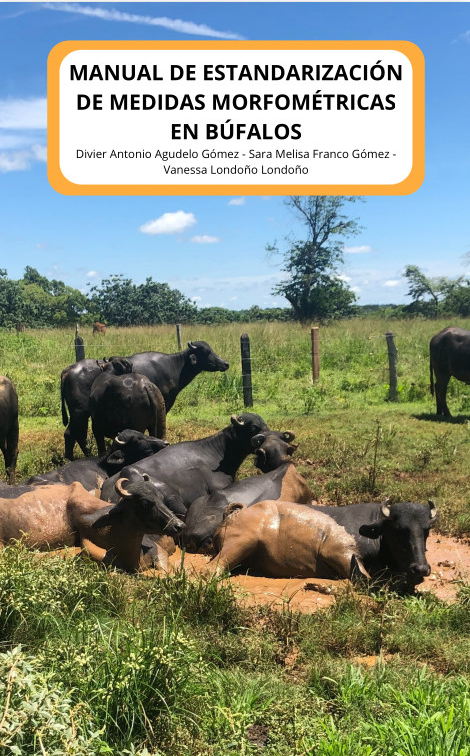
\includegraphics[width=0.6\linewidth]{images/cover} \caption{Portada manual de estandarización para medidas morfométricas en búfalos.}\label{fig:sf-ogc}
\end{figure}

Este manual tiene como objetivo establecer la correcta
toma de medidas morfométricas en ganado bufalino,
con la finalidad de obtener información que apoye los
procesos de selección y mejoramiento genético.
Además, busca facilitar el proceso de toma de medidas
en producciones bufalinas, para que desde productores hasta
investigadores tengan la capacidad de realizar la labor y llevar
a cabo procesos de mejoramiento productivo y reproductivo de manera más
eficiente.

\chapter{Introducción}\label{introducciuxf3n}

En Colombia, la especie Bufalina se introdujo en la década del 60 del Siglo XX, producto de una importación realizada por el INCORA desde Trinidad y Tobago. Estos animales eran inicialmente empleados para trabajo de carga, pero dada la buena adaptación y alta capacidad productiva, reproductiva y longevidad mostrada por la especie, varios productores se enfocaron en producir carne y leche de Búfalo.

Según el censo bufalino realizado en el año 2023 por el ICA (Instituto Colombiano de Agricultura), Colombia cuenta actualmente con un inventario de 485.141 búfalos, distribuidos en 6.033 predios \citep{ICA2022}.

Dado el crecimiento exponencial que ha presentado la especie bufalina en el sector pecuario, se hace indispensable la utilización de herramientas que permitan identificar y describir sus características productivas y reproductivas, para poder implementar procesos de selección y mejoramiento genético más precisos.

La morfometría es una de estas herramientas, y es una disciplina que busca relacionar medidas de la conformación corporal con la capacidad productiva que tiene un grupo de animales \citep{Cardenas2018}, además de representar una ventaja para el productor o criador al permitir identificar los animales para su clasificación, proceso de selección y mejoramiento genético.

\chapter{Objetivos}\label{objetivos}

\section{Objetivo general}\label{objetivo-general}

Desarrollar un manual que funcione como referencia técnica para la realización precisa de medidas morfométricas en ganado bufalino.

\section{Objetivos específicos}\label{objetivos-especuxedficos}

\begin{itemize}
\tightlist
\item
  Identificar los puntos anatómicos entre los que se deben tomar las medidas morfométricas.
\item
  Describir el procedimiento y condiciones básicas para la correcta toma de las medidas morfométricas.
\item
  Indicar las herramientas que se deben utilizar para la toma, registro y análisis adecuado de los datos tomados.
\item
  Establecer un protocolo estandarizado que contribuya a la mejora de la evaluación morfológica y caracterización de esta especie.
\end{itemize}

\chapter{Metodología}\label{metodologuxeda}

El presente trabajo fue descriptivo, ya que su objetivo no fue buscar relación de causa y efecto entre dos eventos, sino instaurar el diseño de un manual en el que se establezca la correcta toma de medidas morfométricas en ganado bufalino, con la finalidad de obtener información que apoye los procesos de selección y mejoramiento.

Este manual cuenta con el nombre de cada medida morfométrica y los puntos anatómicos específicos entre los cuales debe ser tomada. Además, con el objetivo de tener una herramienta visual, se tomaron fotografías guías en las que se van a mostrar dichos lugares anatómicos.

El lugar en el que se llevó a cabo la toma de fotos para el manual es en la finca Villa Elisa, ubicada en el Centro de Veterinaria y Zootecnia de la Facultad de Medicina Veterinaria y Zootecnia de la Universidad CES, con dirección Calle 36 D Sur Kilómetro 4 Loma El Escobero, Envigado, Colombia.

Se trabajó con un solo animal domesticado y dócil, carente de patologías y de alteraciones morfológicas.

El procedimiento se desarrolló de la siguiente forma:

\begin{enumerate}
\def\labelenumi{\arabic{enumi}.}
\tightlist
\item
  Preparación del animal
\item
  Identificación de puntos anatómicos
\item
  Inmovilización del animal
\item
  Toma de medidas morfométricas
\end{enumerate}

\chapter{Marco Teórico y Estado del Arte}\label{marco-teuxf3rico-y-estado-del-arte}

La morfometría es una disciplina que permite relacionar las características anatómicas con características de interés productivo y reproductivo, de tal forma que los procesos de selección y mejoramiento genético sean más precisos \citep{Medina2005}. Esta caracterización permite también conocer las aptitudes de cada especie y raza animal en la que sean tomadas \citep{Gonzalez2021}.

\section{Medidas morfométricas más usadas en ganado bovino}\label{medidas-morfomuxe9tricas-muxe1s-usadas-en-ganado-bovino}

\begin{itemize}
\tightlist
\item
  Altura a la cruz
\item
  Altura al sacro
\item
  Altura a la cadera o a la grupa
\item
  Amplitud de cadera o de grupa
\item
  Amplitud de isquiones
\item
  Amplitud o profundidad de anca
\item
  Longitud corporal
\item
  Longitud de lomo
\item
  Profundidad corporal
\item
  Distancia entre las escápulas
\item
  Perímetro torácico
\item
  Circunferencia testicular o escrotal
\item
  Longitud testicular
\end{itemize}

\section{Instrumentos de medición}\label{instrumentos-de-mediciuxf3n}

\begin{itemize}
\tightlist
\item
  Bastón zoométrico
\item
  Compás de broca
\item
  Cinta métrica o biométrica
\item
  Escrotímetro
\end{itemize}

\section{Estudios previos}\label{estudios-previos}

(Aquí puedes incluir un resumen de los estudios previos mencionados en el documento original)

\chapter{Medidas Morfométricas}\label{medidas-morfomuxe9tricas}

En esta sección, describiremos detalladamente cada una de las medidas morfométricas que se incluirán en el manual.

\section{Altura a la cruz (AC)}\label{altura-a-la-cruz-ac}

La altura a la cruz es la distancia entre la cruz y el extremo distal del miembro anterior. Hace referencia a la estatura del animal entre estos dos puntos anatómicos \citep{Estrada2009}.

(Aquí puedes incluir una imagen ilustrativa)

\section{Altura al sacro (AS)}\label{altura-al-sacro-as}

La altura al sacro es la distancia que existe desde la base del hueso sacro al piso \citep{Vargas}. Está altamente correlacionado con la ganancia de peso en machos. Animales muy altos suelen ser desbalanceados, tener menos carne en canal y presentar problemas de aplomos \citep{Estrada2009}.

(Aquí puedes incluir una imagen ilustrativa)

(Continúa con las demás medidas morfométricas)

\chapter{Consideraciones Éticas}\label{consideraciones-uxe9ticas}

De acuerdo con el Artículo 11 de la Resolución 8430 de 1993, el presente proyecto se clasifica como sin riesgo, ya que se llevó a cabo dentro de las prácticas rutinarias y de manipulación de animales que se realizan en la finca, a las cuales se les atribuye el riesgo mínimo de manipulación más no al proyecto. La toma de medidas morfométricas se hizo con el ejemplar dentro de un brete, para asegurar la correcta sujeción de este y que no existiera riesgo ni para el animal ni para los operarios.

Previo a la toma de medidas y de fotografías, se obtuvo aval del encargado directo del animal, en este caso en específico, la decanatura de la Facultad de Medicina Veterinaria y Zootecnia de la Universidad CES. Las fotografías se tomaron con interés netamente académico, y no se divulgó el nombre de la finca ni el nombre del animal.

\chapter{Resultados Esperados}\label{resultados-esperados}

Con la realización de este proyecto, se busca crear un manual de medidas morfométricas basado en las características morfológicas de la especie bufalina, que se pueda aplicar en todos los predios que manejen ese tipo de ganado; y, además, que sea sencillo y entendible a la lectura, para que desde operarios hasta investigadores adquieran la habilidad de realizar la labor.

Al facilitar la toma de estas medidas morfométricas, se hace más fácil la recopilación de datos para crear una base en la que cada hato pueda fundamentarse al momento de realizar programas de mejoramiento genético, e incrementar el valor productivo y reproductivo de sus ejemplares según las características deseadas.

\chapter{Aplicaciones interactivas}\label{aplicaciones-interactivas}

\subsection{Frecuencia relativa}\label{frecuencia-relativa}

\begin{Shaded}
\begin{Highlighting}[]
\NormalTok{Pc }\OtherTok{\textless{}{-}} \FunctionTok{c}\NormalTok{(}\DecValTok{5}\NormalTok{,}\DecValTok{1}\NormalTok{,}\DecValTok{3}\NormalTok{,}\DecValTok{0}\NormalTok{,}\DecValTok{2}\NormalTok{,}\DecValTok{1}\NormalTok{,}\DecValTok{5}\NormalTok{,}\DecValTok{3}\NormalTok{,}\DecValTok{2}\NormalTok{,}\DecValTok{4}\NormalTok{,}\DecValTok{1}\NormalTok{,}\DecValTok{2}\NormalTok{,}\DecValTok{4}\NormalTok{,}\DecValTok{2}\NormalTok{,}\DecValTok{0}\NormalTok{,}\DecValTok{3}\NormalTok{,}\DecValTok{5}\NormalTok{,}\DecValTok{1}\NormalTok{,}\DecValTok{5}\NormalTok{,}\DecValTok{4}\NormalTok{)}
\NormalTok{Tabla1 }\OtherTok{\textless{}{-}} \FunctionTok{as.data.frame}\NormalTok{(}\FunctionTok{sort}\NormalTok{(}\FunctionTok{table}\NormalTok{(}\AttributeTok{TC3 =}\NormalTok{Pc),}\AttributeTok{decreasing =}\NormalTok{ T))}
\NormalTok{Tabla2 }\OtherTok{\textless{}{-}} \FunctionTok{transform}\NormalTok{(Tabla1, }\AttributeTok{FreAc =} \FunctionTok{cumsum}\NormalTok{(Freq))}
\NormalTok{Tabla3 }\OtherTok{\textless{}{-}} \FunctionTok{transform}\NormalTok{(Tabla2,}\AttributeTok{Rel =} \FunctionTok{round}\NormalTok{(}\FunctionTok{prop.table}\NormalTok{(Freq),}\DecValTok{3}\NormalTok{))}
\NormalTok{knitr}\SpecialCharTok{::}\FunctionTok{kable}\NormalTok{(}
\NormalTok{Tabla3,}
\AttributeTok{caption =} \StringTok{\textquotesingle{}Frecuencia Relativa\textquotesingle{}}\NormalTok{,}
  \AttributeTok{booktabs =} \ConstantTok{TRUE}
\NormalTok{)}
\end{Highlighting}
\end{Shaded}

\begin{table}

\caption{\label{tab:Tabla1}Frecuencia Relativa}
\centering
\begin{tabular}[t]{lrrr}
\toprule
TC3 & Freq & FreAc & Rel\\
\midrule
1 & 4 & 4 & 0.20\\
2 & 4 & 8 & 0.20\\
5 & 4 & 12 & 0.20\\
3 & 3 & 15 & 0.15\\
4 & 3 & 18 & 0.15\\
\addlinespace
0 & 2 & 20 & 0.10\\
\bottomrule
\end{tabular}
\end{table}

\section{Shiny - Estadística}\label{shiny---estaduxedstica}

\begin{verbatim}
## PhantomJS not found. You can install it with webshot::install_phantomjs(). If it is installed, please make sure the phantomjs executable can be found via the PATH variable.
\end{verbatim}

\section{Herramienta para realizar cálculos}\label{herramienta-para-realizar-cuxe1lculos}

\section{Herramienta para realizar gráficas}\label{herramienta-para-realizar-gruxe1ficas}

\section{Herramientas para cálculo estadístico}\label{herramientas-para-cuxe1lculo-estaduxedstico}

\phantomsection\label{ggb-element4}

\section{Herramienta para hoja de cálculo}\label{herramienta-para-hoja-de-cuxe1lculo}

\phantomsection\label{ggb-element1}

  \bibliography{book.bib}

\end{document}
